\documentclass[12pt]{article}
\usepackage{fancyhdr}
\usepackage{amsmath, enumitem, tikz, pgf}
\usepackage{amssymb, amsmath, graphicx, amsthm, setspace}
\usetikzlibrary{arrows, automata, positioning}
\usepackage[latin1]{inputenc}
\pagestyle{fancy}

\lhead[lh-even]{\textbf{Michael Vu}}  
\lfoot[lf-even]{} 
\chead[ch-even]{\textbf{CSCI 3500 HW 3}}  
\cfoot[cf-even]{} 
\rhead[rh-even]{February 27, 2018}  
\rfoot[rf-even]{}

\begin{document}

\begin{enumerate}
\item \quad\\
	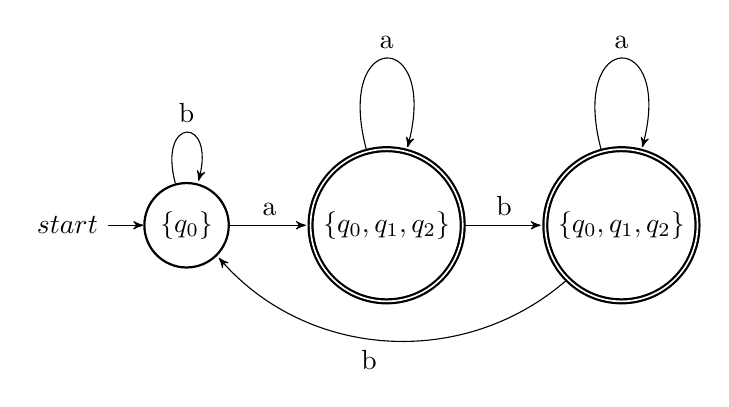
\begin{tikzpicture}
		\tikzset {->, >=stealth', node distance=1cm, every state/.style={thick, fill=none}, initial text=$start$ }
				
		\node[state, initial] (0) {$\{q_0\}$};
		\node[state, right=of 0, accepting] (1) {$\{q_0,q_1,q_2\}$};
		\node[state, right=of 1, accepting] (2) {$\{q_0,q_1,q_2\}$};
			
		\draw[every loop]
			(0) edge[loop above] node {b} (0)
			(0) edge[auto=left] node {a} (1)
			(1) edge[loop above] node {a} (1)
			(1) edge[auto=left] node {b} (2)
			(2) edge[loop above] node {a} (2)
			(2) edge[bend left=45, auto=left] node {b} (0);
	\end{tikzpicture}

\item See attached code.

\item
	\begin{enumerate}
	\item $a(a+b)^*b$
	\item $aaa(a+b)^*$
	\item $000+(0+1)^*+000$
	\item $(aa)^*a$
	\item $(aa)^* + (aaa)^* + (aaaaa)^*$
	\end{enumerate}

\item 
	\begin{enumerate}
	\item Lemma-based construction:

		\bigskip

		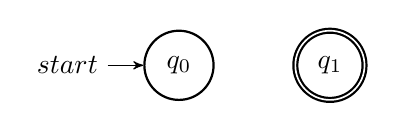
\begin{tikzpicture}
			\tikzset {->, >=stealth', node distance=1cm, every state/.style={thick, fill=none}, initial text=$start$ }
		
			\node[state, initial] (q0) {$q_0$};
			\node[state, accepting, right=of q0] (q1) {$q_1$};
		\end{tikzpicture}

		\bigskip
		
		Smallest construction:
		
		\bigskip

		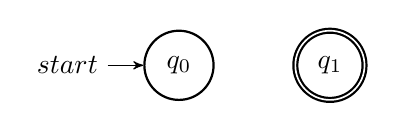
\begin{tikzpicture}
			\tikzset {->, >=stealth', node distance=1cm, every state/.style={thick, fill=none}, initial text=$start$ }
		
			\node[state, initial] (q0) {$q_0$};
			\node[state, accepting, right=of q0] (q1) {$q_1$};
		\end{tikzpicture}
		
	\item Lemma-based construction:

		\bigskip

		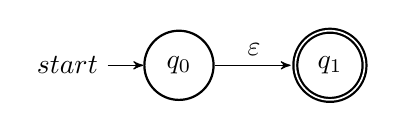
\begin{tikzpicture}
			\tikzset {->, >=stealth', node distance=1cm, every state/.style={thick, fill=none}, initial text=$start$ }
		
			\node[state, initial] (q0) {$q_0$};
			\node[state, accepting, right=of q0] (q1) {$q_1$};
			
			\draw[every loop]
				(q0) edge[auto=left] node {$\varepsilon$} (q1);
		\end{tikzpicture}

		\bigskip
		
		Smallest construction:
		
		\bigskip

		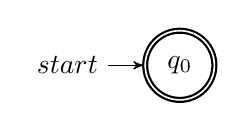
\begin{tikzpicture}
			\tikzset {->, >=stealth', node distance=1cm, every state/.style={thick, fill=none}, initial text=$start$ }
		
			\node[state, initial, accepting] (q0) {$q_0$};
		\end{tikzpicture}
		
	\item Lemma-based construction:

		\bigskip

		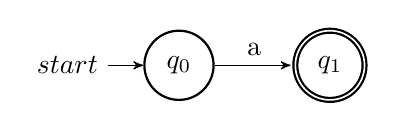
\begin{tikzpicture}
			\tikzset {->, >=stealth', node distance=1cm, every state/.style={thick, fill=none}, initial text=$start$ }
		
			\node[state, initial] (q0) {$q_0$};
			\node[state, accepting, right=of q0] (q1) {$q_1$};
			
			\draw[every loop]
				(q0) edge[auto=left] node {a} (q1);
		\end{tikzpicture}

		\bigskip
		
		Smallest construction:
		
		\bigskip

		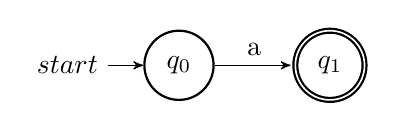
\begin{tikzpicture}
			\tikzset {->, >=stealth', node distance=1cm, every state/.style={thick, fill=none}, initial text=$start$ }
		
			\node[state, initial] (q0) {$q_0$};
			\node[state, accepting, right=of q0] (q1) {$q_1$};
			
			\draw[every loop]
				(q0) edge[auto=left] node {a} (q1);
		\end{tikzpicture}
		
	\item Lemma-based construction:
	
		\bigskip
	
		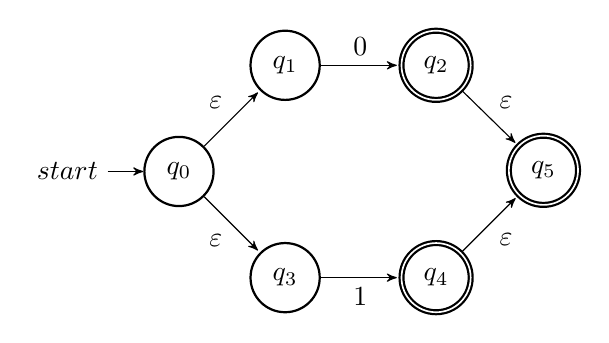
\begin{tikzpicture}
			\tikzset {->, >=stealth', node distance=1cm, every state/.style={thick, fill=none}, initial text=$start$ }
	
			\node[state, initial] (q0) {$q_0$};
			\node[state, above right=of q0] (q1) {$q_1$};
			\node[state, right=of q1, accepting] (q2) {$q_2$};
			\node[state, below right=of q0] (q3) {$q_3$};
			\node[state, right=of q3, accepting] (q4) {$q_4$};
			\node[state, above right=of q4, accepting] (q5) {$q_5$};
			
			\draw[every loop]
				(q0) edge[auto=left] node {$\varepsilon$} (q1)
				(q1) edge[auto=left] node {0} (q2)
				(q2) edge[auto=left] node {$\varepsilon$} (q5)
				(q0) edge[auto=right] node {$\varepsilon$} (q3)
				(q3) edge[auto=right] node {1} (q4)
				(q4) edge[auto=right] node {$\varepsilon$} (q5);
			\end{tikzpicture}
		
			\bigskip
	
		Smallest construction:
	
			\bigskip
		
		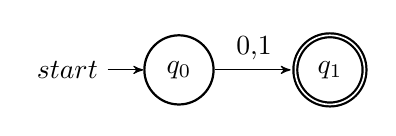
\begin{tikzpicture}
			\tikzset {->, >=stealth', node distance=1cm, every state/.style={thick, fill=none}, initial text=$start$ }
	
			\node[state, initial] (q0) {$q_0$};
			\node[state, right=of q0, accepting] (q1) {$q_1$};
			
			\draw[every loop]
				(q0) edge[auto=left] node {0,1} (q1);
		\end{tikzpicture}
	
	\item Lemma construction:
	
		\bigskip
		
		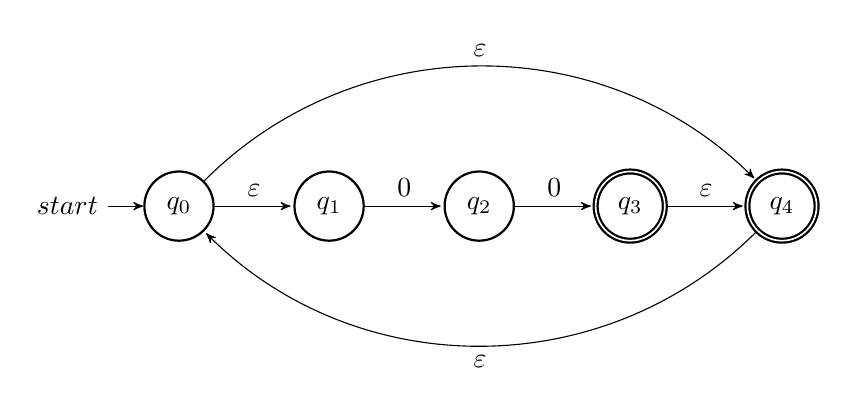
\begin{tikzpicture}
			\tikzset {->, >=stealth', node distance=1cm, every state/.style={thick, fill=none}, initial text=$start$ }
		
			\node[state, initial] (q0) {$q_0$};
			\node[state, right=of q0] (q1) {$q_1$};
			\node[state, right=of q1] (q2) {$q_2$};
			\node[state, right=of q2, accepting] (q3) {$q_3$};
			\node[state, right=of q3, accepting] (q4) {$q_4$};
			
			\draw[every loop]
				(q0) edge[bend left=45, auto=left] node {$\varepsilon$} (q4)
				(q0) edge[auto=left] node {$\varepsilon$} (q1)
				(q1) edge[auto=left] node {0} (q2)
				(q2) edge[auto=left] node {0} (q3)
				(q3) edge[auto=left] node {$\varepsilon$} (q4)
				(q4) edge[bend left=45, auto=left] node {$\varepsilon$} (q0);
		\end{tikzpicture}
		
		\bigskip
		
		Smallest construction:
		
		\bigskip
		
		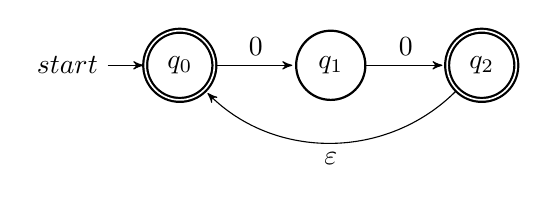
\begin{tikzpicture}
			\tikzset {->, >=stealth', node distance=1cm, every state/.style={thick, fill=none}, initial text=$start$ }
		
			\node[state, initial, accepting] (q0) {$q_0$};
			\node[state, right=of q0] (q1) {$q_1$};
			\node[state, right=of q1, accepting] (q2) {$q_2$};
			
			\draw[every loop]
				(q0) edge[auto=left] node {0} (q1)
				(q1) edge[auto=left] node {0} (q2)
				(q2) edge[bend left=45, auto=left] node {$\varepsilon$} (q0);
		\end{tikzpicture}
		
	\item Lemma construction:
	
		\bigskip
	
		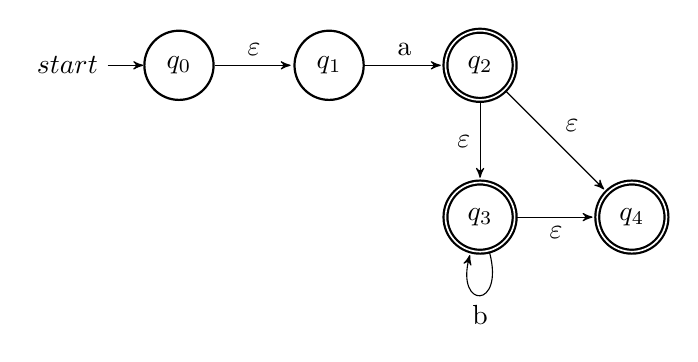
\begin{tikzpicture}
			\tikzset {->, >=stealth', node distance=1cm, every state/.style={thick, fill=none}, initial text=$start$ }
		
			\node[state, initial] (q0) {$q_0$};
			\node[state, right=of q0] (q1) {$q_1$};
			\node[state, right=of q1, accepting] (q2) {$q_2$};
			\node[state, below=of q2, accepting] (q3) {$q_3$};
			\node[state, right=of q3, accepting] (q4) {$q_4$};
			
			\draw[every loop]
				(q0) edge[auto=left] node {$\varepsilon$} (q1)
				(q1) edge[auto=left] node {a} (q2)
				(q2) edge[auto=right] node {$\varepsilon$} (q3)
				(q3) edge[loop below] node {b} (q3)
				(q3) edge[auto=right] node {$\varepsilon$} (q4)
				(q2) edge[auto=left] node {$\varepsilon$} (q4);
		\end{tikzpicture}
		
		\bigskip
		
		Smallest construction:
		
		\bigskip
		
		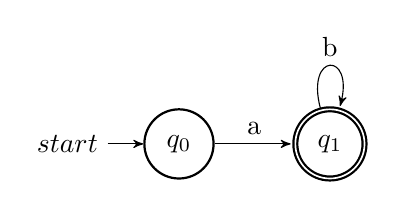
\begin{tikzpicture}
			\tikzset {->, >=stealth', node distance=1cm, every state/.style={thick, fill=none}, initial text=$start$ }
		
			\node[state, initial] (q0) {$q_0$};
			\node[state, right=of q0, accepting] (q1) {$q_1$};
			
			\draw[every loop]
				(q0) edge[auto=left] node {a} (q1)
				(q1) edge[loop above] node {b} (q1);
		\end{tikzpicture}
	\end{enumerate}
\end{enumerate}

\end{document}